\documentclass[
  a4paper,
  12pt,
  parskip=half,
  headings=standardclasses,
  footskip=0pt,
  footlines=1,
  headheight=80in
]{scrartcl}
\setlength{\textheight}{1.15\textheight}

\input{metainfo-include.tex}

\sloppy
\usepackage[utf8]{inputenc}
\usepackage{enumerate}
\usepackage{xcolor}
\usepackage{graphicx}
\usepackage{hyperref}
\usepackage{amsmath}
\usepackage{amssymb}
\usepackage{paracol}
\usepackage{palatino}
\usepackage{mathtools}
\usepackage{listings}
\usepackage[headsepline]{scrlayer-scrpage}
\usepackage[most, listings]{tcolorbox}
\usepackage{longtable}[=v4.13]
\usepackage{tabu}
\usepackage{tikz}
\usetikzlibrary{shapes.misc, positioning}

\definecolor{darkblue}{rgb}{0,0,0.5}
\hypersetup{%
  colorlinks=true,
  urlcolor=darkblue
}

\pagestyle{scrheadings}
\setkomafont{pageheadfoot}{}
\ohead{\small CP 2023}
\ihead{\small Prof.\ Dr.\ Friedrich, Dr.\ Lenzner, Fischbeck, Gawendowicz}
\cfoot{}

\addtolength{\headheight}{-1.5em}

\newcommand{\makeheader}{%
  \columnratio{0.2,0.6,0.2}
  \begin{paracol}{3}
      \switchcolumn
  \center{\Large\textbf{Competitive Programming SS23}}\\
  \vspace{2mm}
  \textbf{Submit until end of contest}
  \switchcolumn
  \hfill
  \includegraphics[width=2.5cm]{hpi-logo.pdf}\\
  \end{paracol}

  \noindent\textbf{Problem: \problemName{}} (\timelimit{} second timelimit) 
}
% \newcommand{\makeheader}{%
%   \columnratio{0.7}
%   \begin{paracol}{2}
%     \begin{leftcolumn}
%       \noindent{\Large\textbf{(Adv.) Competitive Programming}}\\

%       \noindent{\small\textbf{Submit until \deadline{}}}
%     \end{leftcolumn}
%     \begin{rightcolumn}
%       \vspace*{-8mm}
%       \includegraphics[width=4cm]{Hasso_Plattner_Institut_Logo.pdf}
%     \end{rightcolumn}
%   \end{paracol}
%   \vspace*{1em}

%   \noindent\textbf{Problem: \problemName{}} (\timelimit{} second timelimit)
% }

\newcommand{\placeholder}[1]{\textcolor{blue}{#1}}

\newenvironment{samples}[1][1]{%
  \noindent
  \begin{longtabu} to \textwidth {@{}X[#1] X[1]@{}}
    \textbf{Sample input} & \textbf{Sample output} \\
}{%
  \end{longtabu}
}
\newcommand{\sampleBox}[1]{%
  % Using frame=empty doesn't work for listings broken across pages
  \tcbinputlisting{listing file=#1, listing only, colframe=white, colback=black!10!white, sharp corners, box align=top}
}
\newcommand{\sample}[1]{%
  \sampleBox{../testcases/#1.in} & \sampleBox{../testcases/#1.ans} \\
}

\newcommand{\bonusnotice}{%
\textit{Note:} This is a problem that is harder to solve than usual.
Solve the other problems first before spending too much time on this one.

\vspace{1em}
}


\begin{document}

\makeheader

%\placeholder{Problem description}
\textmusicalnote
\emph{You and your rattlegang are hanging out at the park at night}
\textmusicalnote

One of your fellow rattlers starts talking about a cool partner-rattling-workshop taking place next weekend.
Of course the whole gang wants to participate and learn about improving their skills on the rattle,
especially since the workshop focuses on rattling in sync with your rattle-partner. 

Of course partner-rattling is quite complicated and requires a whole lot of trust and mutual understanding of rhythm and music,
so every one of you can only imagine signing up for the workshop with a close friend and mutual rattler. 

However, such a rattlegang is a quite complex and rigid social network.
Every gang member considers themselves either a fan of fast glasses or a mullet maniac.
To never hang out with a friend and having to worry about them having a faster pair of glasses or a more meticulously styled mullet,
every fan of fast glasses is only friends with mullet maniacs and vice versa.
Since a rattle gang needs to be able to operate at any time and without any jealousy every gang member is only permitted to have exactly 3 friends within the gang.

You are wondering what's the largest number of pairs of friends who can sign up for the partner-rattling-workshop. 

\paragraph*{Input}

%\placeholder{Input description}
The first line contains an even number $n$ ($6 \leq n \leq 10^6$), the number of members of the rattle gang.
The following $3 \cdot \frac{n}{2}$ lines contain all friendships within your gang, denoted by two numbers $a$ ($1 \leq a \leq \frac{n}{2}$) and $b$ ($\frac{n}{2} + 1 \leq b \leq n$), indicating that fan of fast glasses $a$ and mullet maniac $b$ are friends.
% No m necessary since the degree of the nodes determines the number of edges, also no need to even read the edges

\paragraph*{Output}

%\placeholder{Output description}
Output a single integer: The largest number of pairs of friends that you can form within your gang in order to participate in the workshop. 

\begin{samples}
  \sample{sample1}
  \sample{sample2}
\end{samples}

\begin{figure}[h]
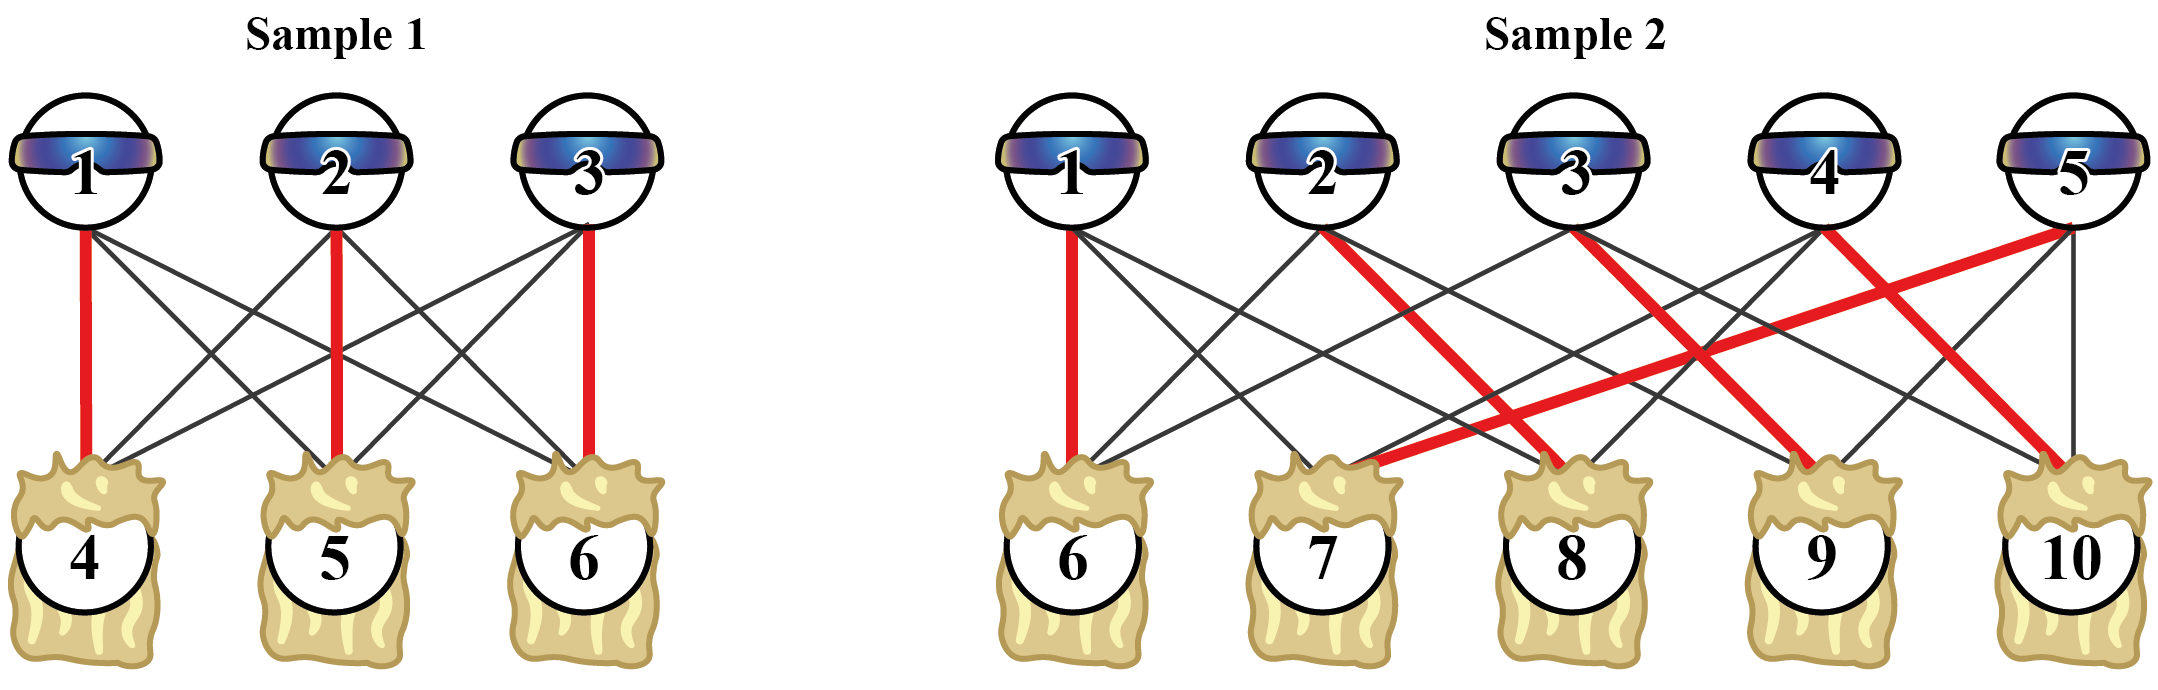
\includegraphics[width=\textwidth]{../../rattlegang.png}
\caption{Visualizations for both sample-rattlegangs. All edges are friendships. The edges highlighted in red show an example of possible pairs for the workshop.}
\end{figure}

\end{document}